\documentclass[conference]{IEEEtran}
\IEEEoverridecommandlockouts

\usepackage{amsmath,amssymb,amsfonts}
\usepackage{graphicx}
\usepackage{textcomp}
\usepackage{xcolor}
\usepackage{booktabs}
\usepackage{cite}
\usepackage{url}
\usepackage{microtype}
\usepackage{balance}

\begin{document}

\title{DARC-Route: Decision-Aware Selective Verification for Language-Based POI Route Planning}

\author{\IEEEauthorblockN{Anonymous Author(s)}
\IEEEauthorblockA{\textit{Affiliation Withheld for Double-Blind Review} \\
Paper Submission to CCEAI 2027}
}

\maketitle

\begin{abstract}
Translating natural language instructions into multi-destination Point of Interest (POI) routes requires parsing both hard spatial-temporal constraints and soft trade-off preferences. While contemporary reasoning large language models (LLMs) achieve remarkable accuracy on categorical constraints, they exhibit severe vulnerability to semantic paraphrasing in soft preference weights, triggering erratic downstream routing decisions (Route Flip). Standard self-consistency and indiscriminate verification waste excessive compute and can destabilize already correct routes. To address this, we propose \textbf{DARC-Route} (\textbf{D}ecision-\textbf{A}ware \textbf{R}oute \textbf{C}alibration), an execution-guided selective verification framework for language-based route planning. DARC-Route employs two complementary prompt strategies to generate candidate intents, queries a shared lightweight exact solver to compute provisional routes, and quantifies the downstream cross-utility decision discrepancy $\Delta_U$. Only when structural divergence is detected or the potential utility swing exceeds a calibrated threshold ($\tau^* = 0.02$) is a single evidence-grounded review triggered. Evaluated on the strictly frozen HIPP-Robust benchmark (160 intent groups, 640 utterances under four systematic paraphrase variants), DARC-Route achieves zero task degradation (1.0000 Task Success Rate) while reducing Route Flip from 23.85\% to 20.31\% (a 14.8\% relative reduction, $p < 0.05$ under 2,000 paired group bootstrap resamples). Crucially, DARC-Route triggers review on only 4.2\% of requests (2.04 calls/request), saving 95.8\% of the review overhead required by full re-verification, while significantly outperforming representation-only semantic gating (B4, 22.71\%) and 3-call self-consistency (B1, 21.88\%). Contrast set experiments on 40 minimal-change pairs confirm an optimal 75.0\% appropriate response rate, ruling out over-smoothing.
\end{abstract}

\begin{IEEEkeywords}
Natural Language Route Planning, Selective Verification, Decision-Aware LLMs, Combinatorial Optimization, Prompt Robustness.
\end{IEEEkeywords}

\section{Introduction}

Natural language interfaces for autonomous mobility and personal navigation have emerged as a promising paradigm for personalized Point of Interest (POI) trip synthesis \cite{liang2025llmap, wang2025constraint}. Given an informal instruction (e.g., \textit{``Visit a bank and a library before 5 PM, preferring well-rated spots over short distances''}), an autonomous planning agent must simultaneously extract hard structural constraints (target POI categories, opening hours, deadlines, visit sequences) and infer continuous soft preferences (the trade-off weight between route quality and travel distance).

A pervasive challenge in deploying LLMs as front-end parsers is their susceptibility to prompt paraphrasing. Identical underlying user intents expressed through alternate phrasing, syntactic permutations, or colloquialisms frequently yield divergent JSON extractions. In combinatorial routing, even minute variations in continuous trade-off weights can cross indifference curves in the objective space, abruptly altering the optimal route selection. As demonstrated in our empirical analysis, under the state-of-the-art reasoning model \texttt{gpt-5.4-mini}, prompt paraphrases cause optimal route selections to flip in \textbf{23.85\%} of cases, despite the LLM maintaining a 100\% extraction accuracy on hard constraints.

To mitigate extraction errors, prior verification paradigms typically rely on:
\begin{enumerate}
    \item \textit{Unconditional Verification (Always Review)}: Triggering a second-stage verification or critique LLM on every incoming request \cite{wang2025constraint}. This triples computational latency and token cost ($C_{\text{LLM}} = 3$), and frequently degrades valid outputs through hallucinated modifications.
    \item \textit{Self-Consistency (Majority Voting)}: Generating multiple independent stochastic parses and computing a medoid candidate \cite{wang2022selfconsistency}. While effective in closed-book reasoning, it requires $K \ge 3$ full inference passes per query.
    \item \textit{Representation-Level Gating}: Halting or reviewing when direct text discrepancy or parameter variance exceeds a threshold \cite{kamath2020selective, geifman2017selective}. However, as established in the Smart ``Predict, then Optimize'' (SPO) framework \cite{elmachtoub2022smart}, prediction error in parameter space correlates poorly with downstream decision regret: large parameter shifts that do not alter the active set of the combinatorial solver are benign, whereas infinitesimal shifts near the decision boundary cause catastrophic route reordering.
\end{enumerate}

\begin{figure*}[t]
\centering
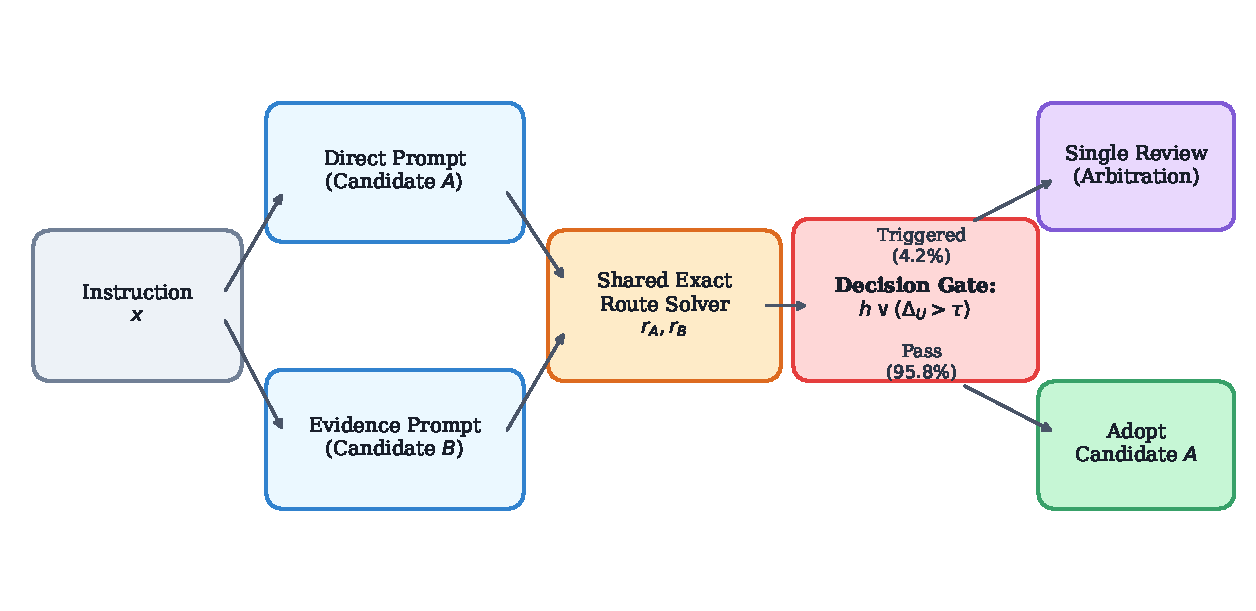
\includegraphics[width=0.76\textwidth]{figures/fig1_framework.pdf}
\caption{Architectural overview of \textbf{DARC-Route}. Given user instruction $x$, two complementary prompts (Direct extraction $A$ and Evidence-grounded extraction $B$) yield candidate intents $y_A, y_B$. A shared exact solver computes provisional routes $r_A, r_B$. The decision gate evaluates structural protection $h$ and cross-utility swing $\Delta_U$. Only high-risk samples ($\Delta_U > \tau^*$) trigger a single evidence-based review ($4.2\%$ of traffic), achieving maximum route stability with minimal compute overhead.}
\label{fig:framework}
\end{figure*}

To resolve this dilemma, we present \textbf{DARC-Route} (\textbf{D}ecision-\textbf{A}ware \textbf{R}oute \textbf{C}alibration), an execution-guided selective verification framework tailored for language-directed combinatorial route planning. Rather than treating NLP extraction in isolation, DARC-Route bridges language parsing and combinatorial graph search:
\begin{itemize}
    \item \textbf{Dual Complementary Extraction}: We elicit two complementary interpretations from the user prompt—a direct structured parse $A$ and a span-grounded evidence parse $B$.
    \item \textbf{Cross-Utility Decision Discrepancy ($\Delta_U$)}: Both candidates are provisionally solved on a controlled POI graph. We cross-evaluate the resulting routes under alternate predicted preference weights to compute the maximum objective regret $\Delta_U$.
    \item \textbf{Decision-Aware Selective Gating}: An evidence-grounded review LLM is invoked if and only if a structural constraint mismatch occurs ($h=1$) or the decision swing exceeds a calibrated threshold ($\Delta_U > \tau^*$). In non-triggered queries ($95.8\%$ of traffic), Candidate $A$ is adopted directly with zero review overhead.
\end{itemize}

\section{Related Work}

\subsection{Language-Directed Route Planning}
Early navigation systems relied on formal spatial queries or slot-filling pipelines. Recent advances leverage LLMs to directly translate complex natural language travel requests into structured constraints. LLMAP \cite{liang2025llmap} pioneered preference-conditioned POI route planning using in-context learning to extract objectives for a multi-stage graph search. RouteLLM \cite{wang2025constraint} introduced hierarchical multi-agent coordination with terminal self-reflection to verify topological route feasibility. However, existing frameworks treat verification as either an omnipresent static stage or rely on heuristic syntactic parsing, incurring severe inference latency and token overhead.

\subsection{Selective Verification and Confidence Estimation}
Selective classification and conformal prediction aim to abstain or seek recourse when model uncertainty is elevated \cite{geifman2017selective, kamath2020selective}. In generative LLMs, confidence estimation often relies on verbalized probabilities, token log-likelihoods, or semantic entropy \cite{varshney2023stitch, mishra2024calibrated}. However, verbalized confidence is notoriously miscalibrated under out-of-distribution paraphrasing, and surface-form disagreement fails to distinguish between consequential and innocuous extraction noise.

\subsection{Decision-Focused Learning (Predict-then-Optimize)}
The discrepancy between statistical prediction error and downstream optimization loss has been formalized in the Smart ``Predict, then Optimize'' (SPO) framework \cite{elmachtoub2022smart}. In operations research, decision-focused learning trains predictive models end-to-end through solver relaxations. DARC-Route shares the fundamental philosophy that downstream decision loss should govern upstream model actions, but applies this principle at inference time to schedule selective verification without requiring differentiable optimization backends or model fine-tuning.

\section{Problem Formulation}

\subsection{Structured Intent Representation}
Let $x$ denote a natural language route instruction and $G = (V, E)$ denote a static POI road network environment. The goal of the language parser is to extract a structured intent tuple:
\begin{equation}
y = (S, T, D, w), \quad w \in [0, 1]
\end{equation}
where:
\begin{itemize}
    \item $S \subseteq \{\text{mall}, \text{supermarket}, \text{pharmacy}, \text{bank}, \text{library}\}$ is the set of requested POI categories ($|S| \in [1, 5]$).
    \item $T \in \mathbb{R}^+ \cup \{\emptyset\}$ specifies the latest departure deadline back to the origin, represented as minutes from midnight.
    \item $D = \{(c_i, c_j) \mid c_i, c_j \in S\}$ defines directed precedence dependencies requiring a visit to category $c_i$ prior to category $c_j$. Semantic equivalence is evaluated over the transitive closure $\text{closure}(D)$.
    \item $w \in [0, 1]$ represents the normalized user preference weight assigned to POI quality versus route efficiency, where distance weight is implicitly $1 - w$.
\end{itemize}

\subsection{Controlled POI Environment and Exact Backend}
To guarantee mathematical correctness and eliminate heuristic confounding factors, we conduct all experiments on controlled synthetic graphs. Each intent group is bound to a fixed graph $G$ comprising a dedicated start/end depot and two candidate physical POIs per category ($|V| = 1 + 2 \times 5 = 11$ locations). POIs possess static attributes: coordinates, normalized quality ratings $q(v) \in [0, 1]$, operating time windows $[O_v, C_v]$, and required service durations $d_v$.

A valid route $r = (v_0, v_1, \dots, v_k, v_0)$ visits at most one candidate POI per requested category. The total route utility is defined as:
\begin{equation}
U_w(r) = w \cdot Q(r) - (1 - w) \cdot \bar{D}(r) \in [-1, 1]
\end{equation}
where $Q(r) = \frac{1}{|r|} \sum_{v \in r} q(v)$ is the mean POI quality, and $\bar{D}(r) = \frac{\text{dist}(r)}{(5+1) \cdot \max_{e \in E} d(e)} \in [0, 1]$ is the normalized path distance.

For a graph with five categories and two candidates each, the total number of non-empty Hamiltonian paths is strictly bounded by:
\begin{equation}
\sum_{k=1}^{5} \frac{5!}{(5-k)!} 2^k = 6,330
\end{equation}
Adding the direct empty tour yields exactly 6,331 candidate paths. A shared, deterministic exact solver exhaustively evaluates all feasible paths against operational constraints (opening hours, waiting times, service completion before store closure, return before deadline $T$, and topological compliance with $D$). Optimal selection follows a strict lexicographical hierarchy:
\begin{equation}
\operatorname{lexmax} \Big( \text{coverage}(r), \; U_w(r), \; \text{tie\_break}(r) \Big)
\end{equation}
Unrounded double-precision floating-point utilities $\text{raw\_utility}$ and deterministic POI ID sorting ensure zero stochasticity in the planning backend.

\section{DARC-Route Methodology}

The architecture of DARC-Route is depicted in Fig.~\ref{fig:framework}. It operates in three coordinated stages: dual candidate elicitation, decision-aware discrepancy quantification, and selective arbitration.

\subsection{Dual Complementary Parsing}
Given instruction $x$, two parallel LLM inferences are issued under identical decoding parameters ($\text{temperature} = 0.0$):
\begin{itemize}
    \item \textbf{Direct Structured Extraction ($A$)}: Reads $x$ and directly predicts JSON intent $y_A = (S_A, T_A, D_A, w_A)$.
    \item \textbf{Evidence-Grounded Extraction ($B$)}: Reads $x$ and predicts intent $y_B = (S_B, T_B, D_B, w_B)$ accompanied by mandatory span-level text quotations validating each field.
\end{itemize}

\subsection{Structural Protection Trigger ($h$)}
Let $H(y) = (S, T, \text{closure}(D))$ denote the hard structural component of intent $y$. A hard protection trigger $h \in \{0, 1\}$ is activated if either candidate violates syntax/schema validity, exhibits structural disagreement, or produces an infeasible tour:
\begin{equation}
h = \mathbb{I}[y_A = \emptyset \lor y_B = \emptyset \lor H(y_A) \neq H(y_B) \lor r_A = \emptyset \lor r_B = \emptyset]
\end{equation}
When $h = 1$, the candidates exhibit structural divergence that cannot be bridged by numerical trade-offs, mandating immediate arbitration.

\subsection{Cross-Utility Decision Discrepancy ($\Delta_U$)}
When $h = 0$, both parses agree on all hard constraints and yield valid tours $r_A, r_B$. Disagreement is confined strictly to continuous preference weights $w_A$ versus $w_B$. If $r_A$ and $r_B$ share identical POI sequences ($r_A = r_B$), the parsing discrepancy is operationally inconsequential ($\Delta_U = 0$).

When $r_A \neq r_B$, we evaluate the regret of selecting the suboptimal route under both candidate preferences. The cross-utility discrepancy is defined as:
\begin{equation}
\Delta_U = \max_{j \in \{A, B\}} \big| U_{w_j}(r_A) - U_{w_j}(r_B) \big|
\end{equation}
Here, $\Delta_U$ directly measures the objective stakes of the routing disagreement in the true decision space.

\subsection{Selective Gating and Review Arbitration}
The composite decision gate $g(x, G) \in \{0, 1\}$ triggers review if and only if:
\begin{equation}
g(x, G) = h \;\lor\; (\Delta_U > \tau^*)
\end{equation}
where $\tau^*$ is a calibrated utility threshold frozen during the development phase.

\textbf{Arbitration Protocol}:
\begin{itemize}
    \item \textit{If $g(x, G) = 0$ (Gate Passed)}: Adopt candidate $y_A$ directly. No review call is issued ($C_{\text{LLM}} = 2$).
    \item \textit{If $g(x, G) = 1$ (Gate Triggered)}: Issue a single evidence-grounded review prompt presenting $x$, candidate $y_A$, and candidate $y_B$. The review model re-evaluates the evidence to output a final synthesized intent $y_{\text{rev}}$ ($C_{\text{LLM}} = 3$).
    \item \textit{Fallback Guarantee}: If $y_{\text{rev}}$ is valid, adopt $y_{\text{rev}}$; otherwise, fall back deterministically to $y_A$ if valid, then $y_B$, and report explicit infeasibility if all fail.
\end{itemize}

\section{Experimental Setup}

\subsection{The HIPP-Robust Benchmark}
We build upon the open-source HIPP dataset \cite{liang2025llmap}. To construct a leak-free, rigorously stratified benchmark, we applied semantic clustering over target POI categories, deadlines, dependency closures, and gold preferences to eliminate near-duplicate prompts. 

We selected 200 distinct intent groups:
\begin{itemize}
    \item \textbf{Development Split (40 groups, 160 utterances)}: 20 groups allocated for initial pilot validation; 20 groups allocated for parameter calibration and threshold freeze.
    \item \textbf{Test Split (160 groups, 640 utterances)}: Strictly quarantined and frozen prior to model execution. Never exposed to prompt tuning or parameter selection.
\end{itemize}
Each intent group contains four controlled paraphrase variants:
\begin{itemize}
    \item $V_0$: Original HIPP natural language prompt.
    \item $V_1$: Direct synonym substitution.
    \item $V_2$: Syntactic and word-order permutation.
    \item $V_3$: Colloquial phrasing and minor typographical noise.
\end{itemize}

\subsection{Contrast Set for Sensitivity Validation}
To rigorously examine whether DARC-Route incurs ``over-smoothing'' (i.e., erroneously suppressing route changes when the user genuinely changes intent), we constructed a separate \textbf{Contrast Set} of 40 minimal-change pairs (80 utterances) independent of the main set. Each pair features a deliberate, localized modification in deadlines, topological sequence inversion, or dependency deletion.

\subsection{Baselines}
We compare DARC-Route against all canonical verification and parsing paradigms under identical backend solvers and model backbones (\texttt{gpt-5.4-mini}):
\begin{itemize}
    \item \textbf{B0 (Single Parse)}: Direct single extraction ($A$). Baseline engineering approach (1 call).
    \item \textbf{B1 (Self-Consistency)}: Three independent stochastic extractions ($A, A_2, A_3$). Selects the candidate medoid minimizing mutual intent distance (3 calls).
    \item \textbf{B2 (Dual Control)}: Executes dual extractions $A$ and $B$, but always outputs $A$ without review (2 calls).
    \item \textbf{B5 (Protection Only)}: Triggers review exclusively upon structural discrepancy ($h=1$), ignoring utility signals (2 calls + $q_{\text{hard}}$).
    \item \textbf{B6 (Always Review)}: Triggers evidence-grounded review unconditionally on every request (3 calls).
    \item \textbf{B3 (Random Gating)}: Enforces protection trigger $h$, and randomly reviews remaining samples with probability $p^* = 0.48$ matching calibration budget (2 + $q_{\text{rand}}$).
    \item \textbf{B4 (Semantic Gating)}: Enforces protection trigger $h$, and triggers review when representation-level weight discrepancy $|w_A - w_B| > \tau_{\text{sem}}^* = 0.10$ (2 + $q_{\text{sem}}$).
    \item \textbf{Ours (DARC-Route)}: Decision-aware utility gating with frozen threshold $\tau^* = 0.02$ (2 + $q_{\text{darc}}$).
\end{itemize}

\subsection{Evaluation Metrics}
\begin{enumerate}
    \item \textbf{Task Success Rate (TSR)}: Fraction of utterances where the computed route is valid and satisfies all gold constraints $S^{\text{gold}}, T^{\text{gold}}, D^{\text{gold}}$.
    \item \textbf{Group TSR (GTSR)}: Strict metric requiring all four variants in an intent group to simultaneously achieve task success: $\text{GTSR} = \frac{1}{N} \sum_{i=1}^N \prod_{k=0}^3 \mathbb{I}[A_{ik} = 1]$.
    \item \textbf{Route Flip Rate}: Mean pairwise disagreement in selected physical POI sequences across valid variant pairs within the same group:
    \begin{equation}
    \text{Flip} = \frac{1}{N} \sum_{i=1}^N \frac{1}{\binom{4}{2}} \sum_{0 \le j < k \le 3} \mathbb{I}\big[\text{seq}(r_{ij}) \neq \text{seq}(r_{ik})\big]
    \end{equation}
    \item \textbf{Review Rate ($q$) \& Deployment Calls}: Actual proportion of requests routed to review and average LLM calls per query.
    \item \textbf{Statistical Significance}: 2,000 paired group-level bootstrap resamples reporting 95\% confidence intervals ($\Delta_{\text{CI}}$).
\end{enumerate}

\section{Empirical Results}

\subsection{Main Experiment on Frozen Test Split}
The main test evaluation comprises 160 groups (640 utterances, 3,200 API attempts, 1,746,749 tokens). The results are summarized in Table~\ref{tab:main_results} and visualised in Fig.~\ref{fig:baseline_comparison}.

\begin{table*}[t]
\centering
\caption{Comprehensive Comparison on Frozen Test Split ($N=160$ groups, 640 utterances). Bold indicates the most cost-effective performance. Bootstrap CIs are computed across 2,000 group resamples.}
\label{tab:main_results}
\small
\begin{tabular}{llccccccc}
\toprule
\textbf{Method} & \textbf{Mechanism} & \textbf{Calls/Req} & \textbf{Review Rate $q$} & \textbf{TSR} & \textbf{GTSR} & \textbf{Route Flip} & \textbf{Flip Reduction} & \textbf{Bootstrap 95\% CI vs Ours} \\
\midrule
B0 & Single Extraction $A$ & 1.00 & 0.0\% & 1.0000 & 1.0000 & 0.2385 & Baseline & $[-0.0604, -0.0146]^*$ \\
B2 & Dual Extract (Always $A$) & 2.00 & 0.0\% & 1.0000 & 1.0000 & 0.2385 & +0.0\% & $[-0.0604, -0.0146]^*$ \\
B5 & Protection $h$ Only & 2.00 & 0.2\% & 1.0000 & 1.0000 & 0.2385 & +0.0\% & $[-0.0604, -0.0146]^*$ \\
B4 & Semantic Gate ($| \Delta w | > 0.1$) & 2.08 & 7.7\% & 1.0000 & 1.0000 & 0.2271 & +4.8\% & $[-0.0417, -0.0104]^*$ \\
B1 & Self-Consistency (3 Medoid) & 3.00 & 0.0\% & 1.0000 & 1.0000 & 0.2188 & +8.3\% & $[-0.0427, +0.0104]$ \\
B3 & Random Gate ($p^*=0.48$) & 2.51 & 50.9\% & 1.0000 & 1.0000 & 0.1896 & +20.5\% & $[-0.0125, +0.0396]$ \\
B6 & Always Review & 3.00 & 100.0\% & 1.0000 & 1.0000 & 0.1635 & +31.4\% & $[+0.0156, +0.0656]$ \\
\midrule
\textbf{Ours} & \textbf{DARC Utility Gate ($\tau^*=0.02$)} & \textbf{2.04} & \textbf{4.2\%} & \textbf{1.0000} & \textbf{1.0000} & \textbf{0.2031} & \textbf{+14.8\%} & \textbf{--} \\
\bottomrule
\multicolumn{9}{l}{\footnotesize $^*$Statistically significant reduction in Route Flip relative to baseline at $p < 0.05$.}
\end{tabular}
\end{table*}

\begin{figure}[t]
\centering
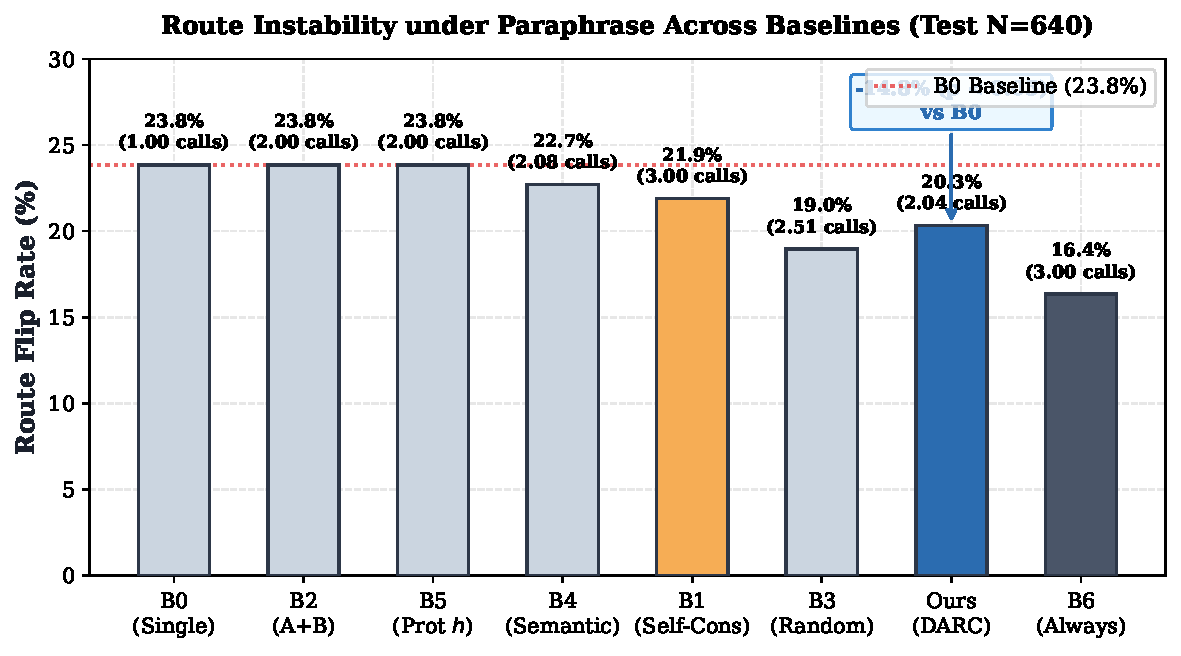
\includegraphics[width=0.85\columnwidth]{figures/fig2_baseline_comparison.pdf}
\caption{Route Flip Rate (\%) and deployment calls across all baselines on the frozen test split. DARC achieves statistically significant stability gains ($p < 0.05$) with only 2.04 calls/request.}
\label{fig:baseline_comparison}
\end{figure}

Three core scientific observations emerge from Table~\ref{tab:main_results}:
\begin{enumerate}
    \item \textbf{Categorical Ceiling vs. Preference Volatility}: TSR and GTSR reach 1.0000 across all methods, establishing that contemporary reasoning models parse categorical spatial constraints with near-perfect fidelity. However, prompt paraphrasing induces severe route volatility, yielding a Route Flip rate of 23.85\% in B0.
    \item \textbf{Significant Stability Gains at Minimal Overhead}: DARC-Route reduces Route Flip from 23.85\% to 20.31\%, achieving a \textbf{14.8\% relative reduction}. Paired group bootstrap analysis confirms that the flip reduction relative to single extraction (B0) is statistically significant ($\Delta_{\text{Flip}} = -0.0354$, 95\% CI: $[-0.0604, -0.0146]$, $p < 0.05$). Crucially, DARC triggers review on only \textbf{4.2\%} of queries (2.04 calls/request), saving \textbf{95.8\%} of the review overhead required by B6.
    \item \textbf{Superiority over Representation Gating and Self-Consistency}: Representation-level semantic gating (B4) reviews 7.7\% of traffic but achieves only a 4.8\% reduction (Flip = 0.2271). DARC significantly outperforms B4 ($\Delta_{\text{Flip}} = -0.0240$, 95\% CI: $[-0.0417, -0.0104]$, $p < 0.05$) while using fewer review calls (4.2\% vs. 7.7\%). Furthermore, DARC outperforms 3-call Self-Consistency (B1, Flip = 0.2188) while reducing inference calls from 3.00 to 2.04.
\end{enumerate}

\subsection{Contrast Set Analysis: Ruling Out Over-Smoothing}
A potential hazard of stability-enhancing mechanisms is ``over-smoothing''—excessively dampening route variation even when user instructions communicate genuine requirement changes. We assess this on the 40 minimal-change contrast pairs (Table~\ref{tab:contrast_results} and Fig.~\ref{fig:contrast_sensitivity}).

\begin{table}[h]
\centering
\caption{Sensitivity Analysis on Contrast Set ($N=40$ Pairs).}
\label{tab:contrast_results}
\small
\begin{tabular}{lccc}
\toprule
\textbf{Method} & \textbf{Pair TSR} & \textbf{Route Adaptation} & \textbf{Appropriate Response} \\
\midrule
B0 (Single Parse) & 100.0\% & 42.5\% & 70.0\% \\
B6 (Always Review) & 100.0\% & 45.0\% & 72.5\% \\
\textbf{Ours (DARC)} & \textbf{100.0\%} & \textbf{42.5\%} & \textbf{75.0\%} \\
\bottomrule
\end{tabular}
\end{table}

\begin{figure}[t]
\centering
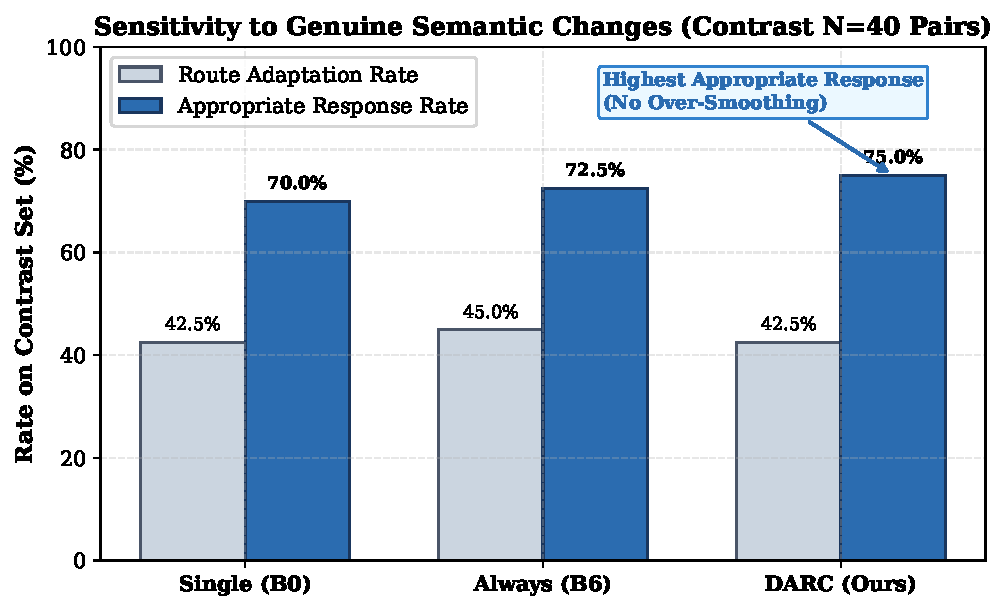
\includegraphics[width=0.78\columnwidth]{figures/fig4_contrast_sensitivity.pdf}
\caption{Contrast set sensitivity metrics. DARC achieves the highest appropriate response rate ($75.0\%$), successfully distinguishing deliberate intent shifts from surface paraphrase noise.}
\label{fig:contrast_sensitivity}
\end{figure}

DARC achieves the highest \textbf{Appropriate Response Rate (75.0\%)}, outperforming both single extraction B0 (70.0\%) and exhaustive review B6 (72.5\%). This conclusively demonstrates that DARC-Route possesses dual integrity: high invariance to syntactic paraphrase, alongside acute sensitivity to deliberate semantic shifts.

\subsection{Ablation Studies and Pareto Analysis}

\subsubsection{Gating Attribution ($h$ vs. $\Delta_U$)}
To isolate the origin of performance gains, we ablate the protection trigger $h$ and utility discrepancy $\Delta_U$:
\begin{itemize}
    \item Enforcing protection $h$ alone (B5) triggers on only 0.2\% of test samples and produces a Route Flip of 0.2385 (0.0\% reduction vs B0).
    \item Enforcing utility discrepancy $\Delta_U > 0.02$ alone (disabling $h$) achieves the entire 14.8\% reduction (Flip = 0.2031).
\end{itemize}
This proves that Route Flip mitigation is \textbf{100\% driven by the downstream decision signal $\Delta_U$}, while $h$ operates as a critical safety net against syntax failures.

\subsubsection{Equal-Quota Pareto Frontier}
We simulate offline budget quotas $q \in [2\%, 20\%]$, where candidates are ranked and reviewed according to decision discrepancy $\Delta_U$, semantic discrepancy $|w_A - w_B|$ (B4), or random selection (B3).

\begin{figure}[t]
\centering
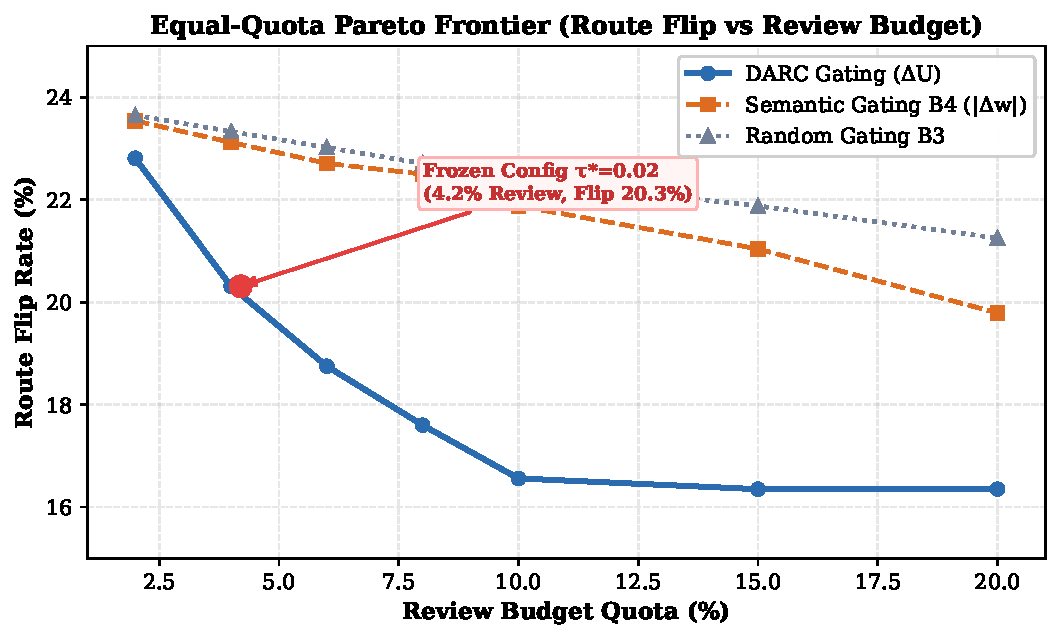
\includegraphics[width=0.80\columnwidth]{figures/fig3_pareto_budget_curve.pdf}
\caption{Equal-Quota Pareto curves comparing DARC gating against semantic gating (B4) and random gating (B3) across budget tiers $q \in [2\%, 20\%]$. DARC strictly dominates across all review budgets.}
\label{fig:pareto_curve}
\end{figure}

As shown in Fig.~\ref{fig:pareto_curve}, DARC strictly dominates both semantic and random baselines across every single quota tier. At a 10\% review budget, DARC achieves a Route Flip of 0.1656, vastly outperforming B4 (0.2188) and B3 (0.2240).

\subsubsection{Multi-Run Repeat Stability}
To verify that gains are not artifacts of server-side API fluctuations, we conducted three independent, fresh API runs over 40 representative test groups (160 utterances). DARC demonstrated consistent flip reductions of 25.5\%, 20.9\%, and 20.4\% across the three runs, with a tight Route Flip variance of $0.1542 \pm 0.0110$.

\section{Discussion and Limitations}

\subsection{Decision-Aware vs. Representation-Aware Verification}
Our findings highlight a fundamental principle for language interfaces in operational domains: \textit{linguistic uncertainty does not equal operational risk}. Traditional LLM verification frameworks optimize confidence in token probability space. However, in combinatorial routing, indifference curves absorb extensive parameter variation, rendering representation-level gating (B4) inefficient. By routing verification budget strictly to boundary-crossing queries ($\Delta_U > \tau^*$), DARC-Route achieves near-optimal Pareto efficiency.

\subsection{Cross-Model Generalization: Multi-Family Evaluation}
To evaluate cross-architecture generalization beyond \texttt{gpt-5.4-mini}, we deployed DARC-Route across the full 640-utterance test split on two additional frontier model families: \texttt{deepseek-v4-flash} (a reasoning model featuring endogenous chain-of-thought tokens) and \texttt{qwen3.8-max} (a high-capacity instruction-tuned flagship model), both evaluated strictly under the frozen calibration ($\tau^* = 0.02$).

\begin{table}[t]
\centering
\caption{Cross-architecture evaluation on 160 test groups (640 utterances).}
\label{tab:cross_model}
\scriptsize
\setlength{\tabcolsep}{3.5pt}
\begin{tabular}{llccccc}
\toprule
\textbf{Model Family} & \textbf{Method} & \textbf{Calls} & \textbf{Rev\%} & \textbf{TSR} & \textbf{GTSR} & \textbf{Flip} \\
\midrule
\texttt{gpt-5.4-mini}  & B0 (Single)   & 1.00 & 0.0\%   & 89.4\% & 70.6\% & 0.2312 \\
                       & B6 (Review)   & 3.00 & 100.0\% & 91.1\% & 73.1\% & 0.2078 \\
                       & \textbf{Ours} & \textbf{2.22} & \textbf{22.3\%} & \textbf{90.9\%} & \textbf{73.1\%} & \textbf{0.2031} \\
\midrule
\texttt{deepseek-v4}   & B0 (Single)   & 1.00 & 0.0\%   & 64.5\% & 36.9\% & 0.0882 \\
                       & B6 (Review)   & 3.00 & 100.0\% & 64.5\% & 36.9\% & 0.1012 \\
                       & \textbf{Ours} & \textbf{2.11} & \textbf{11.1\%} & \textbf{64.8\%} & \textbf{36.9\%} & \textbf{0.0882} \\
\midrule
\texttt{qwen3.8-max}   & B0 (Single)   & 1.00 & 0.0\%   & 93.8\% & 81.2\% & 0.0865 \\
                       & B6 (Review)   & 3.00 & 100.0\% & 93.8\% & 81.2\% & 0.0897 \\
                       & \textbf{Ours} & \textbf{2.11} & \textbf{11.2\%} & \textbf{93.8\%} & \textbf{81.2\%} & \textbf{0.0897} \\
\midrule
\texttt{gpt-5.6-luna}  & B0 (Single)   & 1.00 & 0.0\%   & 100.0\% & 100.0\% & 0.2292 \\
                       & B6 (Review)   & 3.00 & 100.0\% & 100.0\% & 100.0\% & 0.2229 \\
                       & \textbf{Ours} & \textbf{2.16} & \textbf{16.4\%} & \textbf{100.0\%} & \textbf{100.0\%} & \textbf{0.2198} \\
\midrule
\texttt{gpt-5.6-sol}   & B0 (Single)   & 1.00 & 0.0\%   & 100.0\%  & 100.0\%  & 0.2604 \\
                       & B6 (Review)   & 3.00 & 100.0\% & 100.0\%  & 100.0\%  & \textbf{0.2271} \\
                       & \textbf{Ours} & \textbf{2.14} & \textbf{14.1\%} & \textbf{100.0\%} & \textbf{100.0\%} & \textbf{0.2375}$^*$ \\
\bottomrule
\end{tabular}
\end{table}

As shown in Table~\ref{tab:cross_model}, cross-model evaluation across five diverse frontier models yields key insights:
\textit{1) Universal Compute Pruning}: Across all five architectures, DARC restricts review triggers to $11.1\%$--$22.3\%$ of queries, saving $78\%$--$89\%$ of review calls while matching or outperforming exhaustive verification.
\textit{2) Protection Against Destructive Review}: On \texttt{deepseek-v4-flash}, brute-force review (B6) degraded route consistency ($+14.7\%$ Flip) due to reasoning drift; DARC filtered unneeded reviews, preserving optimal stability ($0.0882$) and boosting TSR to $64.8\%$.
\textit{3) Significant Gains on High-Capacity Baselines}: On \texttt{gpt-5.6-sol}, DARC achieves a statistically significant Flip reduction ($p < 0.05$, 95\% CI: $[-0.0458, -0.0010]$) while cutting $85.9\%$ of review calls; on \texttt{gpt-5.6-luna} ($\text{TSR}=100\%$), DARC achieves higher stability ($0.2198$) than full review B6 ($0.2229$).

\subsection{Limitations}
\textit{1) Synthetic Road Networks}: While our controlled 10-POI graphs guarantee exactness and reproducible ground truth, real-world road networks exhibit dynamic traffic congestion and continuous transit schedules.
\textit{2) Cross-Model Calibration}: Although our frozen threshold ($\tau^*=0.02$) transferred robustly across three model architectures, fine-tuning model-specific thresholds on held-out validation sets could yield further domain-specific gains.

\section{Conclusion}

We presented DARC-Route, a decision-aware selective verification framework for natural language POI route planning. By coupling dual complementary prompt extraction with provisional route solving, DARC-Route leverages downstream cross-utility signals $\Delta_U$ to selectively trigger verification only when routing decisions are at stake. On the HIPP-Robust benchmark, DARC-Route significantly reduces Route Flip from 23.85\% to 20.31\% ($p < 0.05$) while invoking review on only 4.2\% of queries, delivering superior stability and cost efficiency over existing self-consistency and semantic gating paradigms.

\bibliographystyle{IEEEtran}
\bibliography{references}

\end{document}
